%% Support sites:
%% http://www.michaelshell.org/tex/ieeetran/
%% http://www.ctan.org/tex-archive/macros/latex/contrib/IEEEtran/
%% and
%% http://www.ieee.org/

% Also note that the "draftcls" or "draftclsnofoot", not "draft", option
% should be used if it is desired that the figures are to be displayed in
% draft mode.
%
\documentclass[conference]{IEEEtran}
% Add the compsoc option for Computer Society conferences.

%\usepackage{ifpdf}
\usepackage{cite}


% *** GRAPHICS RELATED PACKAGES ***
%
\ifCLASSINFOpdf
  % \usepackage[pdftex]{graphicx}
  % declare the path(s) where your graphic files are
  % \graphicspath{{../pdf/}{../jpeg/}}
  % and their extensions so you won't have to specify these with
  % every instance of \includegraphics
  % \DeclareGraphicsExtensions{.pdf,.jpeg,.png}
\else
  % or other class option (dvipsone, dvipdf, if not using dvips). graphicx
  % will default to the driver specified in the system graphics.cfg if no
  % driver is specified.
  % \usepackage[dvips]{graphicx}
  % declare the path(s) where your graphic files are
  % \graphicspath{{../eps/}}
  % and their extensions so you won't have to specify these with
  % every instance of \includegraphics
  % \DeclareGraphicsExtensions{.eps}
\fi
% graphicx was written by David Carlisle and Sebastian Rahtz. It is
% required if you want graphics, photos, etc. graphicx.sty is already
% installed on most LaTeX systems. The latest version and documentation can
% be obtained at:
% http://www.ctan.org/tex-archive/macros/latex/required/graphics/
% Another good source of documentation is "Using Imported Graphics in
% LaTeX2e" by Keith Reckdahl which can be found as epslatex.ps or
% epslatex.pdf at: http://www.ctan.org/tex-archive/info/
%
% latex, and pdflatex in dvi mode, support graphics in encapsulated
% postscript (.eps) format. pdflatex in pdf mode supports graphics
% in .pdf, .jpeg, .png and .mps (metapost) formats. Users should ensure
% that all non-photo figures use a vector format (.eps, .pdf, .mps) and
% not a bitmapped formats (.jpeg, .png). IEEE frowns on bitmapped formats
% which can result in "jaggedy"/blurry rendering of lines and letters as
% well as large increases in file sizes.
%
% You can find documentation about the pdfTeX application at:
% http://www.tug.org/applications/pdftex

\usepackage[cmex10]{amsmath}


% *** SPECIALIZED LIST PACKAGES ***
%
%\usepackage{algorithmic}
% algorithmic.sty was written by Peter Williams and Rogerio Brito.
% This package provides an algorithmic environment fo describing algorithms.
% You can use the algorithmic environment in-text or within a figure
% environment to provide for a floating algorithm. Do NOT use the algorithm
% floating environment provided by algorithm.sty (by the same authors) or
% algorithm2e.sty (by Christophe Fiorio) as IEEE does not use dedicated
% algorithm float types and packages that provide these will not provide
% correct IEEE style captions. The latest version and documentation of
% algorithmic.sty can be obtained at:
% http://www.ctan.org/tex-archive/macros/latex/contrib/algorithms/
% There is also a support site at:
% http://algorithms.berlios.de/index.html
% Also of interest may be the (relatively newer and more customizable)
% algorithmicx.sty package by Szasz Janos:
% http://www.ctan.org/tex-archive/macros/latex/contrib/algorithmicx/

\usepackage{listings}


\usepackage{array}
\usepackage{mdwmath}
\usepackage{mdwtab}

\usepackage{eqparbox}
\usepackage[tight,footnotesize]{subfigure}
%\usepackage[caption=false]{caption}
\usepackage[caption=false, font=footnotesize]{subfig}
% subfig.sty, also written by Steven Douglas Cochran, is the modern
% replacement for subfigure.sty. However, subfig.sty requires and
% automatically loads Axel Sommerfeldt's caption.sty which will override
% IEEEtran.cls handling of captions and this will result in nonIEEE style
% figure/table captions. To prevent this problem, be sure and preload
% caption.sty with its "caption=false" package option. This is will preserve
% IEEEtran.cls handing of captions. Version 1.3 (2005/06/28) and later
% (recommended due to many improvements over 1.2) of subfig.sty supports
% the caption=false option directly:
%\usepackage[caption=false,font=footnotesize]{subfig}
%
% The latest version and documentation can be obtained at:
% http://www.ctan.org/tex-archive/macros/latex/contrib/subfig/
% The latest version and documentation of caption.sty can be obtained at:
% http://www.ctan.org/tex-archive/macros/latex/contrib/caption/




% *** FLOAT PACKAGES ***
%
%\usepackage{fixltx2e}
% fixltx2e, the successor to the earlier fix2col.sty, was written by
% Frank Mittelbach and David Carlisle. This package corrects a few problems
% in the LaTeX2e kernel, the most notable of which is that in current
% LaTeX2e releases, the ordering of single and double column floats is not
% guaranteed to be preserved. Thus, an unpatched LaTeX2e can allow a
% single column figure to be placed prior to an earlier double column
% figure. The latest version and documentation can be found at:
% http://www.ctan.org/tex-archive/macros/latex/base/



%\usepackage{stfloats}
% stfloats.sty was written by Sigitas Tolusis. This package gives LaTeX2e
% the ability to do double column floats at the bottom of the page as well
% as the top. (e.g., "\begin{figure*}[!b]" is not normally possible in
% LaTeX2e). It also provides a command:
%\fnbelowfloat
% to enable the placement of footnotes below bottom floats (the standard
% LaTeX2e kernel puts them above bottom floats). This is an invasive package
% which rewrites many portions of the LaTeX2e float routines. It may not work
% with other packages that modify the LaTeX2e float routines. The latest
% version and documentation can be obtained at:
% http://www.ctan.org/tex-archive/macros/latex/contrib/sttools/
% Documentation is contained in the stfloats.sty comments as well as in the
% presfull.pdf file. Do not use the stfloats baselinefloat ability as IEEE
% does not allow \baselineskip to stretch. Authors submitting work to the
% IEEE should note that IEEE rarely uses double column equations and
% that authors should try to avoid such use. Do not be tempted to use the
% cuted.sty or midfloat.sty packages (also by Sigitas Tolusis) as IEEE does
% not format its papers in such ways.





% *** PDF, URL AND HYPERLINK PACKAGES ***
%
%\usepackage{url}
% url.sty was written by Donald Arseneau. It provides better support for
% handling and breaking URLs. url.sty is already installed on most LaTeX
% systems. The latest version can be obtained at:
% http://www.ctan.org/tex-archive/macros/latex/contrib/misc/
% Read the url.sty source comments for usage information. Basically,
% \url{my_url_here}.





% *** Do not adjust lengths that control margins, column widths, etc. ***
% *** Do not use packages that alter fonts (such as pslatex).         ***
% There should be no need to do such things with IEEEtran.cls V1.6 and later.
% (Unless specifically asked to do so by the journal or conference you plan
% to submit to, of course. )


% correct bad hyphenation here
\hyphenation{op-tical net-works semi-conduc-tor}

\usepackage[normalem]{ulem}
\usepackage{tikz}
\usepackage{xcolor}
\usepackage{lipsum}
\usetikzlibrary{shapes,arrows}

\tikzstyle{decision} = [diamond, draw, fill=blue!20, text width=4.5em,
text badly centered, node distance=3cm, inner sep=0pt]

\tikzstyle{block} = [rectangle, draw, fill=blue!20, text width=5em,
text centered, rounded corners, minimum height=4em]

\tikzstyle{line} = [draw, -latex'] \tikzstyle{cloud} = [draw,
ellipse,fill=red!20, node distance=3cm, minimum height=2em]

\newcommand{\XXX}[1]{{\bf \color{red} XXX: #1}}
\newcommand\reduline{\bgroup\markoverwith
  {\textcolor{red}{\rule[-0.5ex]{2pt}{0.4pt}}}\ULon}
\newcommand{\FIC}[1]{\reduline{#1}}

%\usepackage[margin=1cm]{caption}

\begin{document}

\captionsetup{width=2cm}

\lstdefinestyle{aspectp}{ breaklines=true, frame=tb, morekeywords={},
  xleftmargin=2em, numbers=left, captionpos=b,
  morekeywords={aspectdef, where, when, what} }

\lstdefinestyle{MaxC}{language=C++, breaklines=true, frame=tb,
  xleftmargin=2em, numbers=left,
  captionpos=b,basicstyle=\ttfamily\footnotesize,
  morekeywords={s_int32, int32, float8_24, sin_float8_24,
    sout_float8_24, float8_24, s_int, s_float8_24, s_bool}}

\lstdefinestyle{MaxCconf}{language=C++, xleftmargin=2em,
  morekeywords={kernels, flow, Host, Memory} }

\title{MaxC: Aspect Driven Compilation for \\ Dataflow Designs}

\author{
  \IEEEauthorblockN{
    \emph{Paul Grigoras},
    \emph{Xinyu Niu},
    \emph{Jos\'{e} Gabriel F. Coutinho} and
    \emph{Wayne Luk}}
  \IEEEauthorblockA{
    Department of Computing, Imperial College London, 180 Queen's Gate, London SW7 2AZ, UK \\
    Email: \{paul.grigoras09, niu.xinyu10, gabriel.figueiredo, w.luk\}@imperial.ac.uk}}

\maketitle


\begin{abstract}

  The dataflow model of computation is a convenient paradigm for
  expressing high-throughput parallel computations. It enables
  synthesis of deeply pipelined hardware architectures directly from a
  program's dataflow graph. Dataflow designs can be conveniently
  implemented on Field Programmable Gate Arrays which combine the
  advantage of fully customizable logic with low time to
  market. However, the manual development process used until now is
  challenging, error-prone and counter-productive. We propose a design
  flow that uses aspects to decouple design development from design
  optimisation, thus improving maintainability, portability and
  developer productivity while enabling automated exploration of
  design trade-offs that can lead to increased performance. The
  proposed approach uses MaxC, a novel language for specifying
  dataflow designs. In this paper we introduce MaxC and show how
  inputs, outputs, computation and control parts of hardware designs
  can be captured with high-level MaxC descriptions, and simulated in
  software using the standard GCC stack. Optimisation strategies for
  the generated designs are then specified with LARA, a
  domain-specific aspect oriented programming language, and MaxC. We
  evaluate our approach by developing an implementation for a high
  performance application based on Reverse-Time Migration
  (RTM). Preliminary results show that our design achieves comparable
  performance to state of the art FPGA implementations, \FIC{while
  improving developer productivity}.

\end{abstract}

\IEEEpeerreviewmaketitle

\section{Introduction}

The dataflow computing paradigm is more suitable for implementing high
throughput, highly parallel applications that operate on large amounts
of uniform data than general purpose architectures. Existing work
shows that dataflow machines emulated on FPGAs achieve performance
gains of up to several orders of magnitude compared to traditional
control based architectures \cite{Flynn:Pell:Mencer:2012},
\cite{Mencer:2012},
\cite{Oriato:Tilbury:Marrocu:Pusceddu:2012}. Because they eliminate
the fetch-decode-execute cycle of traditional von Neumann machines
\cite{Neumann:1993}, dataflow designs require less area for caching
and control (e.g. branch prediction) which leads to the increase in
performance and decrease in power consumption. Another key aspect is
that due to its regularity, a dataflow design can be statically
scheduled into a deep hazard-free pipeline, effectively achieving the
ideal throughput rate of one result per clock cycle. This makes
dataflow designs more suitable for expressing high throughput, regular
computations than general purpose computing devices. However, dataflow
languages are not commonly used and even with the advent of more
modern functional programming languages, imperative languages such as
Java and C/C++ remain most popular \cite{Tiobe:2012}.

We identify the following challenges that should be overcome to
facilitate the adoption of dataflow designs:
\begin{enumerate}
\item Specifying dataflow designs, in an intuitive, well understood
  language that is concise and facilitates the translation of existing
  designs and expressive enough to support the requirements of modern
  high-performance applications.
\item Specifying optimization strategies, decoupled from the
  application code in a manner that makes the specification easy to
  reuse and customize and is comprehensive enough to allow capturing
  of optimizations at various levels: \emph{algorithmic
    transformations} that enable transformation of the original
  application to expose parallelism or improve communication between
  CPU and accelerator, \emph{design-level transformations} that
  enable exploration of platform specific optimizations and
  \emph{productivity related transformations} that improve developer
  productivity.
\item Systematic design space exploration of dataflow designs driven
  by these parameterizable optimization strategies, that increase
  developer productivity and allow exploration of design level
  trade-offs.
\item Applying these design techniques to create and optimize high
  performance applications from existing implementations
\end{enumerate}

We propose a methodology for addressing these challenges based on the
following contributions:
\begin{enumerate}
\item We introduce MaxC, a dataflow language based on C99 that can be
  used to create high-performance designs. We implement a compiler
  that translates MaxC designs to MaxJ an existing commercial dataflow
  language. These are then compiled using MaxCompiler 2012.1 and
  executed on a MAX3424 Board with a Virtex 6 FPGA chip and 48GB of
  on-board DRAM.
\item We introduce novel aspects for specifying optimisation
  strategies at the algorithmic level, the design level and
  productivity level. We implement these aspects using
  LARA, an aspect oriented language for FPGA systems.
\item We propose an automated method for design space exploration of
  MaxC dataflow designs, driven by the aspect definitions.
\item We evaluate our approach implementing a high performance design
  for an application based on the Reverse Time Migration technique for
  seismic imaging and comparing it with existing CPU, GPU and FPGA
  implementations.
\end{enumerate}



\section{Design Flow}

The proposed design flow is illustrated in Figure
\ref{fig:design-flow}. MaxC is used to specify dataflow
designs. Transformations specified through aspects are applied to the
original design, generating new MaxC designs. These are then compiled
by the MaxC backend to generate MaxJ design for hardware or
simulation.

The design space exploration process can be automated and ran until a
dataflow design that achieves timing closure and meets non functional
requirements is generated.  For each optimization strategy in our
repository we:

\begin{enumerate}

\item apply the set of specific low-level optimizations comprised in
  the strategy (e.g. setting DSP balance).

\item  we compile the optimized
  design using the MaxCC backend to MaxJ

\item we start the backend compilation toolchain (MaxCompiler
  and Xilinx) and perform an analysis of the reporting information,
  based on which we either restart the flow with the next optimization
  strategy step or proceed to the next step

\item we measure NFRs such as performance or latency and if our target
  is not met we restart using a different optimization strategy

\end{enumerate}
\begin{comment}
  \begin{figure}[!h]
    \caption{The proposed design flow.}
    \begin{center}
      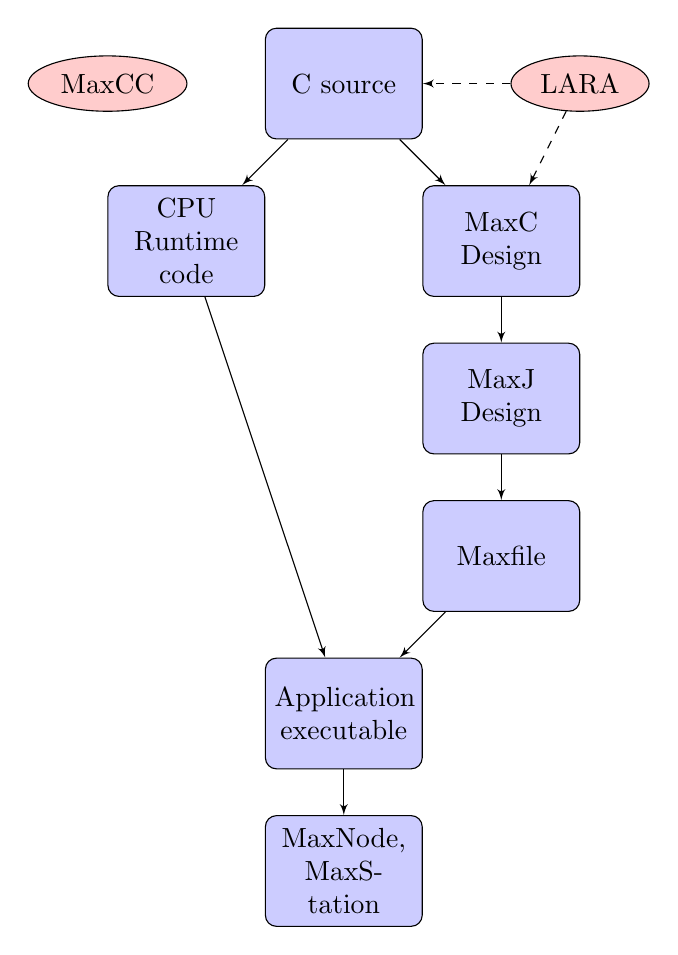
\begin{tikzpicture}[node distance = 2cm, auto, scale=0.5]
        \node [block] (csrc) {C source};
        \node [block, below of=csrc, left of=csrc] (maxrt) {CPU Runtime code};
        \node [block, below of=csrc, right of=csrc] (maxc) {MaxC Design};
        \node [block, below of=maxc] (maxj) {MaxJ Design};
        \node [block, below of=maxj] (maxfile) {Maxfile};
        \node [block, below of=maxfile, left of=maxfile] (app) {Application executable};
        \node [block, below of=app] (maxnode) {MaxNode, MaxStation};

        \node [cloud, right of=csrc] (lara) {LARA};
        \node [cloud, left of=csrc] (maxcc) {MaxCC};
        % \node [cloud, right of=init] (system) {system};
        % \node [block, below of=init] (identify) {identify candidate models};
        % \node [block, below of=identify] (evaluate) {evaluate candidate models};
        % \node [block, left of=evaluate, node distance=3cm] (update) {update model};
        % \node [decision, below of=evaluate] (decide) {is best candidate better?};
        % \node [belock, below of=decide, node distance=3cm] (stop) {stop};

        \path [line] (csrc) -- (maxrt);
        \path [line] (csrc) -- (maxc);
        \path [line] (maxc) -- (maxj);
        \path [line] (maxj) -- (maxfile);
        \path [line] (maxfile) -- (app);
        \path [line] (maxrt) -- (app);
        \path [line] (app) -- (maxnode);
        \path [line, dashed] (lara) -- (csrc);
        \path [line, dashed] (lara) -- (maxc);

        % \path [line] (decide) -| node [near start] {yes} (update);
        % \path [line] (update) |- (identify);
        % \path [line] (decide) -- node {no}(stop);
        % \path [line,dashed] (expert) -- (init);
        % \path [line,dashed] (system) -- (init);
        % \path [line,dashed] (system) |- (evaluate);
      \end{tikzpicture}
    \end{center}
  \end{figure}
\end{comment}

\begin{figure}[!h]
  \includegraphics[scale=0.5, trim=50 180 0 50]{lara_maxcc.pdf}
  \caption{The proposed design flow.}
  \label{fig:design-flow}
\end{figure}


\section{The  MaxC Language}

MaxC is a novel language for specifying dataflow designs. It is based
on the widely used C99 standard which makes it familiar and easy to
adopt for developers facilitating translation of existing application
code to dataflow designs. The simple syntax of C99 facilitates
integration with other tools (such as aspect weavers), allowing the
language to interact well with existing compilers or source to source
translation frameworks (e.g. LARA, ROSE), allowing source level
optimizations to be applied through different tools. MaxC itself is a
simple language, which is intended to be used for expressing the
simplest form of a dataflow design. Optimizations and other
transformations are encapsulated in aspects which are developed
separately and applied through aspect weaving. This results in a more
flexible approach for generating and exploring the space of efficient
dataflow designs.

\begin{comment}
  We identify the following requirements for any dataflow language:
  \begin{enumerate}
  \item intuitive and easy to use
  \item facilitate translation of existing applications
  \item interacts well with
    high-level tools
  \end{enumerate}
\end{comment}

Since MaxC is compiled to MaxJ it uses the same execution model: a
design is composed of one or more computational kernels (which
implement the functionality we are interested in) which are connected
to form a design. Communication between kernels is asynchronous, so
kernels can operate independently of each other but computation within
kernels is synchronous, so a kernel will compute only when all it's
active inputs have values available.

Figure \ref{fig:maxc-1dconv} shows an example MaxC dataflow kernel
which implements a 1D convolution computation used to value European
options.


\lstset{style=MaxC}

\begin{figure}
  \begin{lstlisting}
    void kernel_Convolution1D(float* p, float c_0_0_0, float c_p_0_0, float c_n_0_0, int n1, int ORDER, float* out)
    {

      in(p);

      float* i4 = count(1000, 1);
      float* i1 = countChain(n1, 1, i4);

      #pragma maxc DSPBalance:full
      int result =
      p[0]  * c_0_0_0 +
      p[1]  * c_p_0_0 +
      p[-1] * c_n_0_0;

      int up = (i1 >= ORDER) && (i1 < n1 - ORDER);

      out = up ? result : p;

      out(out);
    }
  \end{lstlisting}
  \caption{Example MaxC design for a 1D convolution kernel.}
  \label{fig:maxc-1dconv}
\end{figure}

\subsection{Kernels}

Kernels are defined as regular C functions, with the ``kernel\_''
identifier prepended (Line 1). The inputs and outputs of the kernel
are clearly specified in the header, inputs followed by outputs. At
the kernel level MaxC captures the dataflow elements by using:

\begin{itemize}
\item \emph{regular C constructs} are used as much as possible to make
  the language more intuitive. This includes standard C99 types and
  conventions for implementing kernels. Some overloaded operators are
  provided such as the array access operators to provide a more
  succinct syntax for accessing ``past'' or ``future'' stream elements
  (Lines 15 -- 17).

\item \emph{pragma directives} are used to convey additional
  information to the compiler for which C99 does not provide flexible
  built-in constructs (e.g. specifying type width) or additional
  optimization hints (e.g. the DSP balance, Line 13);

\item \emph{specific API calls} are used for higher level constructs
  such as inputs and outputs (Lines 8, 24), counters (Lines 10 -- 11).

\end{itemize}


Figure \ref{fig:maxc-1dconv} shows the main elements of a MaxC design:

\begin{enumerate}
\item \emph{inputs and outputs} are declared in the kernel header and
  connected in the kernel body. Lines 2-6 show the kernel declaration
  specifying the stream input "p" and output "out" as well as a number
  of scalar parameters configurable at run-time. API calls are used to
  connect these inputs (Line 7 and 22);

\item \emph{control} elements are implemented either via standard C99
  constructs (such as conditional statements or operators) or via API
  calls that enable multiplexing between 2 or more streams;

\item \emph{computation} is implemented using regular C99 syntax and
  semantics. The MaxCC backend will also automatically translate
  standard functions in the C99 math library to hardware blocks for
  common functions such as square root, exponential, logarithms.

\item \emph{streams} are represented as regular C99 pointers. For
  example Line 2 declares a stream of float values names ``p''.
  Normal array notation can be used to generate either previous
  (negative indices) or future values (positive indices) or
  dereference the stream to get the current stream value. Negative
  indices are allowed (as on Line 16). On lines 13-16 we use array
  index notation to access future (positive offset) or past (negative
  offset) stream elements. Supported offset expressions are linear
  expressions comprised of constants or variables (either loop
  induction variables, or normal variables but for which a compile
  time range of values is specified -- this is required to generate
  efficient hardware).

\item \emph{compile time constructs} such as loops are supported as
  long as their bounds are known at compile time.

\item \emph{optimizations} can be applied via pragmas (Line 12) or API
  calls. Additional type information can also be provided via pragmas.

\end{enumerate}

The MaxC API provides a number of useful, higher-level constructs.
such as output functions that are used to connect an internal kernel
stream to the output stream of a kernel, various counters and counter
chain configurations that can be instantiated using functions from the
counter API (Lines 9 -- 10) or functions such as stream\_select that
are used to multiplex between a number of streams based on the value
of condition stream.


\subsection{Designs}

MaxC also allows specification of designs using multiple kernels. This
involves selecting the kernel instances and connecting them as well as
setting a number of design configuration and compilation options such
as operating frequency.

Figure \ref{lst:maxc-design} illustrates the design for the 1D
convolution example which places and connects memory command kernels
to control the generation of memory streams and the actual computation
kernels.

On Lines 3-6 we specify the kernel instances. On Lines 8 -- 10 we
connect these. Lines 13 -- 15 specify the design frequency, the memory
clock frequency and enable the addition of debug elements.

\begin{figure}[!h]
  \centering
  \begin{lstlisting}
    void design_Convolution1D() {
      // kernels
      kernel_t k1 = kernel_init(kernel_Convolution1D);
      kernel_t k2 = kernel_init(kernel_Cmdwrite);
      kernel_t k3 = kernel_init(kernel_Cmdread);

      // connections
      connect2(k1, k2);
      connect3(k1, k2, ``a'');
      connect4(k1, k3, ``a'', ``b'');

      // configuration
      set_frequency(150);
      set_memory_frequency(333);
      set_enable_debug(true);
    }
  \end{lstlisting}
  \caption{MaxC design specification, connecting multiple kernels and
    setting various configuration options}
  \label{lst:maxc-design}
\end{figure}


\section{Aspects}

MaxC was designed to integrate with aspect weaving tools by using
standard C99 syntax. This allows MaxC specifications to describe the
simplest form of a dataflow design while aspects specify decoupled
optimization and transformation strategies that operate on this
design. This make the functionality of the application easier to
understand, more maintainable and portable since it is no longer
obscured by various structural or algorithmic transformations or
platform specific optimizations.

We distinguish four categories of aspects: \emph{system aspects},
\emph{exploration aspects}, \emph{implementation aspects} and
\emph{development aspects}

\subsection{System Aspects}

System aspects capture transformation or optimization strategies that
affect the whole application such as those concerning
hardware/software portioning, or run-time reconfiguration
capabilities. The goal is to expose parallelism, improve communication
between CPU and accelerator via hardware/software partitioning or
remove idle functions from the accelerator using run-time
reconfiguration. These aspects act on the original C application level
as well as on the partitioned C (software) and MaxC design (hardware).


\subsubsection{\TODO Reconfiguration}

\subsection{Exploration aspects}

Exploration deal with strategies that generate multiple designs based
on parametrisation and can act on any level of the design flow (C
code, C and MaxC, or MaxC design). They enable systematic exploration
of trade-offs and. An example LARA aspect for design space exploration
is show below. It highlights the feedback capabilities of the design
flow: the aspect will generate a MaxC designs and build the DFE
configuration until this passes a specified LUT threshold, at each
step increasing the parallelism of the design (by replicating the
computational pipeline).

\begin{lstlisting}
  aspectdef DSEStrategy
  var config = { 'Dsp_factor': 1,
    'Exponent'  : 8,
    'Mantissa'  : 24 };
  var par = 0, lut_threshold = 10000;
  do {
    par++;
    config['Par'] = par;
    var designName = genName(config);
    call genMaxC(designName, config);
    buildMaxC(designName);
  } while (@hw[designName].lut < lut_threshold);
  end
\end{lstlisting}

\subsection{Implementation Aspects}

Design aspects capture low level design optimizations that can be
applied to the MaxC designs in order to improve timing or explore
various resource usage trade-offs.

Aspects can be used to enable design space exploration of resource
usage vs. accuracy trade-offs by varying the word
lengths. Alternatively we can use them to explore resource trade-offs
by mapping computation to specialised FPGA blocks. For example, the
aspect in Figure \ref{fig:aspect-DSP} can be used to map arithmetic
expressions to DSP blocks. We define the DSP balance factor to be used
(none, normal, full), the granularity (which decides if we break up
arithmetic expressions to insert DSP Factors between them) and the
number of independent applications.

\lstset{style=aspectp}
\begin{figure}[!h]
  \centering
  \begin{lstlisting}
    aspectdef OptimizeDSPUsage(
    DSPBalance, granularity, applications)
    {
      where: arithmetic expression occurs
      what:
      split expression if it has more than granularity operations
      insert DSP balance pragma
    }
  \end{lstlisting}
  \caption{Aspect for exploring mapping of computation to DSP blocks.}
  \label{fig:aspect-DSP}
\end{figure}

Aspects steps:

\begin{enumerate}
\item Identify arithmetic expressions;
\item Split them according to granularity;
\item Insert annotation to adjust DSP usage;
\item Repeat for a given number of applications.
\end{enumerate}

\newsavebox{\secondlisting}
\begin{lrbox}{\secondlisting}% Store second listing
  \lstinputlisting[firstline=8]{code.txt}
\end{lrbox}

\begin{figure}
  \begin{lstlisting}
    #pragma balanceDSP=full
    int result = p[0]  * c_0_0_0;
    int result = result + p[1]  * c_p_0_0;
    #pragma balanceDSP=full
    int result = result + p[-1] * c_n_0_0;
  \end{lstlisting}
  \caption{One possible result of applying
    \texttt{OptimizeDSPUsage(full, fine, 2)} to Lines 13 -- 17 of Figure
    \ref{fig:maxc-1dconv}.}
  \label{fig:maxc-1dconv-aspect}
\end{figure}

Figure \ref{fig:maxc-1dconv-aspect} shows one of the possible results
of applying the aspect \texttt{OptimizeDSPUsage(full, fine, 2 } to
Lines 13 -- 17 of Figure \ref{fig:maxc-1dconv}.

Using LARA we can implement and combine these aspects to enable
systematic design space exploration of all the optimisations options
exposed by the MaxC backend resulting in the generation of a large
number of designs. The feedback-directed compilation process of LARA can
be used to capture and extract feedback from the backend reports
pertaining to resource usage or timing information and automatically
adjust the compilation process.

\subsection{Development Aspects}

Development aspects capture transformations that have an impact on the
development process such as debugging, simulating kernels or improving
compilation speed. Separating these concerns makes the original
application code easier to maintain and enables the automatic
application of these transformations to a wide range of designs, thus
improving developer productivity.

\subsubsection{Simulation Aspects}

The goal for the MaxC kernel simulation model is that it should be
possible to compile and run dataflow designs using the standard GCC
toolchain in order to verify the logical correctness of the
design. However, this often leads to the need of adding boilerplate
code that would otherwise not be required by the MaxC backend, just to
enable simulation. Since this process is itself manual and hence
error-prone it defeats the very purpose of testing the design. One
approach would be to require users to always use the simulation
API. However this unnecessarily complicates the dataflow design. Our
solution is to use separate aspects to generate the simulation
designs.

Simulation aspects can be applied to the original dataflow design to
enable pure software simulation. This approach gives more freedom when
designing MaxC constructs -- since we are not necessarily concerned
weather they compile using the standard GCC toolchain. This in turn
allows us to provide a neater syntax but also hides and automates the
details of generating simulation designs from the developer.

Aspect steps:

\begin{enumerate}

\item insert kernel simulation loop in hostcode %(Figure )
  \begin{figure}[!h]
    \begin{lstlisting}
      for (int i = 0 ; i < CYCLE_COUNT; i++) {
        kernel_Convolution1d(p, out, 2);
        update_stream_pointers(p, out);
      }
    \end{lstlisting}
    %\caption{Stream simulation loop.}
    %\label{fig:maxc-simulation}
  \end{figure}

\item insert boilerplate code in the dataflow design to enable simulation.
  % The result of applying the simulation aspect to the dataflow in
  %  Figure \ref{fig:maxc-1dconv} is shown in Figure
  %  \ref{fig:maxc-sim-aspect}.
  For example any stream and counter used in the kernel body need to
  be declared using special calls that also pass in unique identifiers
  which are used to store and retrieve the values at each cycle in a
  separate data structure (e.g. \texttt{`stream\_init\_i(int
    stream\_id)}). On each kernel cycle, the function then either
  allocates a new stream or increments the stream pointer if the
  stream has already been allocated.
  \begin{comment}
    \begin{figure}[!h]
      \begin{lstlisting}
        float* i4 = count_i(1000, 1, 0);
        float* i1 = countChain_i(n1, 1, i4, 0);
      \end{lstlisting}
      \caption{Applying the simulation aspect to the dataflow design in
        Figure \ref{fig:maxc-1dconv}}
      \label{fig:maxc-sim-aspect}
    \end{figure}
  \end{comment}

\end{enumerate}

\lstset{style=MaxC}


\subsubsection{Debug Aspects}

Because the current execution model does not provide for runtime
debugging of hardware designs the easiest solution to debug designs is
to log the values of various streams during execution. The insertion
of debug statements can be encapsulated in aspects. It is particularly
important to separate debug aspects from the original application code
since debug blocks can influence the compilation time and timing
constraints as well as the behaviour of the design.

\lstset{style=aspectp}
\begin{figure}[!h]
  \centering
  \begin{lstlisting}
    aspectdef DebugValues()
    {
      where: variable assignment
      what:
      log value before assignment
      log value after assignment
    }
  \end{lstlisting}
  \caption{Aspect for exploring mapping of computation to DSP blocks.}
  \label{fig:aspect-DSP}
\end{figure}

\subsubsection{Compilation Aspects}

Compilation aspects can be applied during the development process to
create versions of the dataflow design that compile faster. They apply
changes such as reducing the operating frequency, removing debug
blocks or applying design-level optimizations that can resolve timing
constraints. Naturally reducing the compilation time increases
developer productivity.

Different compilation aspects can be used to build in parallel more
versions of the application that allow incremental testing (in order
of compilation times):
\begin{enumerate}
\item Fastest design to build will be a naive version, optimized for
  compile time (minimum design and memory frequency, disabled debug
  blocks, no arithmetic optimizations). This allows verifying
  application correctness;
\item The debug version (enabled debug blocks) is built in parallel to
  allow debugging of errors identified in the previous step;
\item Finally a version optimized for performance (maximum frequency,
  no debug block, arithmetic optimisations) is compiled to allow
  testing of non-functional requirement.
\end{enumerate}

\section{Evaluation}

\begin{comment}

  \begin{table*}
    %  \renewcommand{\arraystretch}{1.3}
    \centering
    \caption{Results of aspect transformations on the original MaxC
      design for the RTM kernel.}
    \label{table:feature-comparison}
    \begin{tabular}{ p{2cm}  | p{1cm} | c|  p{1cm} |  p{1cm} |  p{1cm} |  p{1cm} | c | p{1cm} |c | c | c}
      Aspect                           & DSP Balance    & Par & LUT               & FF                & BRAM           & DSP            & Frequency & Compile Time & LOC & Speedup & Throughput \\ \hline
      \multirow{4}{*}{OptimizeDSPUsage} & none           & 1   & 67327 (22.62\%)   & 92607  (15.56\%)  & 248 (23.31\%)  & 0  (0.00\%)    & 303/100   & 2 h 9        & LOC & Speedup & Throughput \\
      & balanced       & 1   & 59202 (19.89\%)   & 84101 (14.13\%)   & 248 (23.31\%)  & 34 / (1.69\%)  & 303/100   & 1h 49        & LOC & Speedup & Throughput \\
      & full           & 1   & 52619  (17.68\%)  & 76107  (12.79\%)  & 248  (23.31\%) & 117  (5.80\%)  & 303/100   & 2 h 2        & LOC & Speedup & Throughput \\ \hline
      & none           & 2   & 92109 (30.95\%)   & 122224 (20.53\%)  & 261 (24.53\%)  & 0 (0.00\%)     & 303/100   & 3h5          & LOC & Speedup & Throughput \\
      & balanced       & 2   & 75719 (25.44\%)   & 75719 (25.44\%)   & 261 (24.53\%)  & 68 (3.37\%)    & 303/100   & 2h30         & LOC & Speedup & Throughput \\
      & full           & 2   & 63032  (21.18\%)  & 89284  (15.00\%)  & 260  (24.44\%) & 234  (11.61\%) & 303/100   & 2 h 8        & LOC & Speedup & Throughput \\
      \hline
      & none           & 3   & 116532 (39.16\%)  & 152406 (25.61\%)  & 256 (24.06\%)  & 0 (0.00\%)     & 303/100   & 3 h 20       & LOC & Speedup & Throughput \\
      & balanced       & 3   & 93911 (31.56\%)   & 126888 (21.32\%)  & 256 (24.06\%)  & 102 (5.06\%)   & 303/100   & 2h30         & LOC & Speedup & Throughput \\
      & full           & 3   & 74575  (25.06\%)  & 102965  (17.30\%) & 255  (23.97\%) & 351  (17.41)\% & 303/100   & 2 h 18       & LOC & Speedup & Throughput \\
      \hline
      & \TODO none     & 6   & 116532 (39.16\%)  & 152406 (25.61\%)  & 256 (24.06\%)  & 0 (0.00\%)     & 303/100   & 3 h 20       & LOC & Speedup & Throughput \\
      & \TODO balanced & 6   & 92109 (30.95\%)   & 122224 (20.53\%)  & 261 (24.53\%)  & 0 (0.00\%)     & 303/100   & 3h5          & LOC & Speedup & Throughput \\
      & full           & 6   & 106033  (35.63\%) & 143508  (24.11\%) & 295  (27.73\%) & 702  (34.82\%) & 303/100   & 3h 42        & LOC & Speedup & Throughput \\
    \end{tabular}
  \end{table*}

  \begin{table*}
    % \renewcommand{\arraystretch}{1.3}
    \centering
    \caption{Results of aspect transformations on the original MaxC
      design for the RTM kernel.}
    \label{table:feature-comparison}
    \begin{tabular}{ p{2cm}  | p{1cm} | c|  p{1cm} |  p{1cm} | p{1cm} |   p{1cm} |  p{1cm} | c | p{1cm} |c | c | c}
      Aspect                               & Word Width & Burst & Par & LUT               & FF                & BRAM                 & DSP             & Frequency & Compile Time & LOC & Speedup & Throughput \\ \hline
      \multirow{4}{*}{Optimize word width} & 8, 24      & 64    & 2   & 63447  (21.32\%)  & 89150  (14.98\%)  & 260  (24.44\%))      & 234  (11.61\%)  & 400/100   & 2 h 30       & LOC & Speedup & Throughput \\
      & 8, 24      & 64    & 3   & 75676  (25.4\%)   & 102831  (17.28\%) & 255  (23.97\%)       & 351  (17.41\%)  & 400/100   & 2 h 35       & LOC & Speedup & Throughput \\
      & 8, 24      & 64    & 6   & 101578  (34.13\%) & 143374  (24.09\%) & 248          295  (27.73\%) & 702  (34.82\%)  & 400/100   & 4 h 17       & LOC & Speedup & Throughput \\ \hline
      & 8, 24      & 1     & 6   & 106033  (35.63\%) & 143508  (24.11\%) & 295  (27.73\%)       & 702  (34.82\%)  & 303/100   & 3h 42        & LOC & Speedup & Throughput \\
      & 8, 22      & 1     & 6   & 133973  (45.02\%) & 185520  (31.17\%) & 295  (27.73\%)       & 306  (15.18\%)  & 303/100   & 3 h 13       & LOC & Speedup & Throughput \\
      & 8, 20      & 1     & 6   & 129581  (43.54\%) & 178333  (29.96\%) & 289  (27.16\%)       & 306  (15.18\%)  & 303/100   & 3 h 30       & LOC & Speedup & Throughput \\ \hline
      & 8, 18      & 1     & 6   & 121439  (40.81\%) & 170721  (28.68\%) & 286  (26.88\%)       & 306  (15.18\%)) & 303/100   & 3h 19        & LOC & Speedup & Throughput \\
      & 8, 16      & 1   & 6   & 117904  (39.62\%) & 157359  (26.44\%) & 283  (26.60\%)       & 204  (10.12\%)  & 400/100   & 2 h 50       & LOC & Speedup & Throughput \\ \hline

    \end{tabular}
  \end{table*}
\end{comment}


\subsection{RTM}
We evaluate the proposed approach by implementing a high-performance
application based on the Reverse Time Migration method for seismic
imaging. This models the propagation of injected waves using the
isotropic acoustic wave equation \cite{araya2011assessing}. We
approximate the differential equation using stencil computation to
perform a fifth-order Taylor expansion in space and first-order Taylor
expansion in time.

\subsection{Results}
We use MaxC to implement the dataflow kernel and aspects to
generate multiple configurations for the design.

Results of the design space exploration using the word length aspect
illustrate the trade-offs between accuracy and resource usage.  We
observe irregular, large variations when decreasing the mantissa from
18 16 and 24 to 22. The latter difference is unexpected, halving the
number of required DSPs (although increasing the LUT and FF usage by
30\%), with little impact on accuracy. This is the effect of the
backend tools implementing arithmetic operations using a combination
of both DSPs and LUT/FF elements. The mantissa boundaries at which
this optimization occurs are platform specific (depending on the
architecture of the DSPs). Hence automating this optimization via
aspects and decoupling it from the original source code makes the
application more portable and facilitates discovery of interesting
trade-off opportunities using design space exploration.


\begin{table}[!h]
  %  \renewcommand{\arraystretch}{1.1}
  \centering
  \caption{Results of varying the word length.}
  \label{table:aspect-wl}
  \begin{tabular}{ p{1cm} p{1cm} p{1cm} p{1cm} p{1cm}  p{1cm} }
    Word Width & LUT               & FF                & BRAM           & DSP             & Relative Error \\ \hline
    8, 24      & 106033  (35.63\%) & 143508  (24.11\%) & 295  (27.73\%) & 702  (34.82\%)  & \TODO          \\
    8, 22      & 133973  (45.02\%) & 185520  (31.17\%) & 295  (27.73\%) & 306  (15.18\%)  & \TODO          \\
    8, 20      & 129581  (43.54\%) & 178333  (29.96\%) & 289  (27.16\%) & 306  (15.18\%)  & \TODO          \\
    8, 18      & 121439  (40.81\%) & 170721  (28.68\%) & 286  (26.88\%) & 306  (15.18\%)  & \TODO          \\
    8, 16      & 117904  (39.62\%) & 157359  (26.44\%) & 283  (26.60\%) & 204  (10.12\%)  & \TODO          \\
  \end{tabular}
\end{table}

Design space exploration using the parallelism aspect can be used to
illustrate design scalability. Figure \ref{fig:scalability} shows that
performance scales linearly with the number of parallel
pipelines. This type of exploration can also be used to expose
bottlenecks. This aspect can be combined with others such as adjusting
memory and stream frequency to understand the combined effect of these
optimizations. This would be useful in investigating the trade-off of
performance versus compilation time. In particular, it is not always
necessary to use maximum stream or memory frequency (e.g. in the case
of memory or compute bound applications respectively) but this can
significantly increase compilation time.

\begin{figure}[!h]
  \centering
  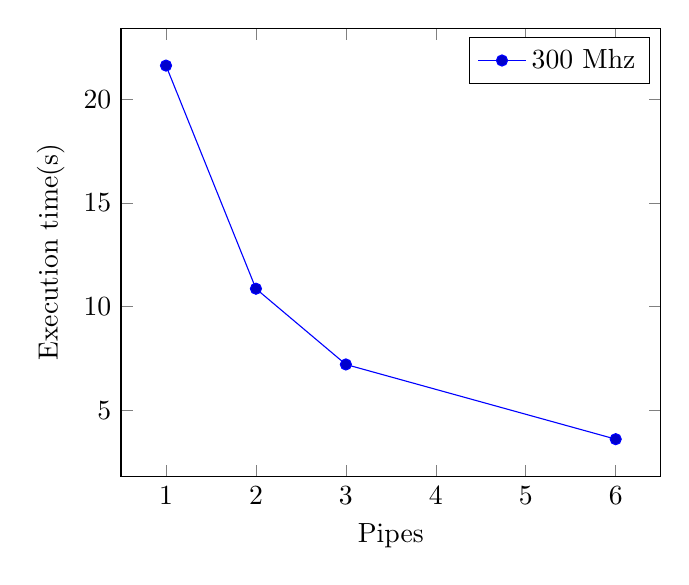
\begin{tikzpicture}
    \begin{axis}[xlabel=Pipes,ylabel=Execution time(s)]
      \addplot coordinates {
        (1, 21.630226)
        (2, 10.86542)
        (3, 7.210907)
        (6, 3.606188)
      };
      \legend{300 Mhz, 333 Mhz. 400 Mhz}
    \end{axis}
  \end{tikzpicture}
  \caption{Scalability of the MaxC dataflow design -- performance
    increases linearly with the number of parallel pipelines.}
  \label{fig:scalability}
\end{figure}


The DSP aspect allows to explore the resource trade-offs of
implementing arithmetic operations in either DSPs or LUTs and
FFs. This can help avoiding over mapping on DSPs for arithmetic
intensive applications.


Finally table \ref{speedup} shows speedups obtained by the MaxC
dataflow design compared to CPU, GPU and other FPGA
implementations. This shows that our approach can match the
performance of the static reference version achieving a significant
speedup of up to 50x over software only versions.

\begin{table}[!h]
  %  \renewcommand{\arraystretch}{1.1}
  \centering
  \caption{Speed up results compared to CPU, GPU and other FPGA implementations. Size s = 128x128x128.}
  \label{speedup}
  \begin{tabular}{ ccccc}
    Size & Pipes & Time  & vs CPU & Throughput (GFlop/s) \\ \hline
    s    & 6     & 3.60  & 50.4X  & 61                   \\
    s    & 3     & 7.21  & 25.2X  & 30.5                 \\
    s    & 2     & 10.86 & 16.7X  & 15.2                 \\
    s    & 1     & 21.63 & 8.4X   & 7.6                  \\\hline
    m    & 6     & -     & -      & -                    \\
    m    & 3     & -     & -      & -                    \\
    m    & 2     & -     & -      & -                    \\
    m    & 1     & -     & -      & -                    \\ \hline
    l    & 6     & -     & -      & -                    \\
    l    & 3     & -     & -      & -                    \\
    l    & 2     & -     & -      & -                    \\
    l    & 1     & -     & -      & -                    \\
  \end{tabular}
\end{table}








\section{Related Work}

\subsection{Dataflow Languages}


Given the advantage that dataflow architectures have when implementing with
uniform computation over general purpose-architecture, it is no
surprise that a number of dataflow language have been developed
targeting FPGAs but also multi-core platforms.

\begin{itemize}

\item Streams-C\cite{Gokhale:Stone:Arnold:Kalinowski:2000} and
  ImpulseC\cite{ImpulseC} (commercial version of Streams-C) use a model based on
  Communicating Sequential Process. Streams-C designs are specified
  using non-standard syntax such as special comment blocks which is
  used to annotate C application code.

\item StreamIt\cite{Thies:Karczmarek:Amarasinghe:2002} and Sequoia++
  use a different, non-standard syntax which is not intuitive for new
  users. This also complicates the translation process of existing
  imperative code.

\item MaxJ \cite{MaxelerTechnologies:2012} is a commercial
  implementation which provides a Java API for constructing dataflow
  designs. However, since the runtime library is C this means that
  developers have to manage two separate project components which
  complicates both interaction between them (e.g. if common design
  parameters are to be shared) and the design space exploration
  process. Additionally Java is a more verbose language and in most
  designs this is not necessarily useful since we don't always benefit
  that from high-level constructs. In C we can use macros to capture
  repetitive patterns, but since C is not an Object Oriented language,
  it can be considerably wore in terms of code reuse.

\end{itemize}

\subsection{Aspect Driven Design}


\subsection{Comparison with Other Dataflow Languages}

Table \ref{table:feature-comparison} summarizes the features of MaxC
in comparison with other languages described in the related works
section.

\begin{table}[!h]
  \renewcommand{\arraystretch}{1.3}
  \centering
  \caption{Feature comparison of MaxC and other dataflow languages.}
  \label{table:feature-comparison}
  \begin{tabular}{ l | c |  p{1cm} |  p{1cm} |  c |  c }
    Language  & Syntax & FPGA Support & Execution Model & Debugging & Simulation \\ \hline
    MaxJ      & -      & -            & -               & -         & -          \\
    Streams-C & -      & -            & -               & -         & -          \\
    ImpulseC  & -      & -            & -               & -         & -          \\
    StreamIt  & -      & -            & -               & -         & -          \\
    Sequoia++ & -      & -            & -               & -         & -          \\
    MaxC      & -      & -            & -               & -         & -          \\
  \end{tabular}
\end{table}


\begin{comment}
  \subsubsection{Translation}

  Translation aspects tranform high-level source code to MaxC designs.

  Aspect steps:
  \begin{enumerate}

  \item identify acceleration candidates by profiling the
    computation. In particular analyse loops with computations and
    profile at various degrees of nesting;

  \item transform local arrays to dynamic arrays;

  \item extract computational kernel by mapping the outer loop to the
    stream loop;

  \item generate runtime API (currently using MaxCompilerRT).

  \end{enumerate}

  This aspect will map the C99 application shown in Figure
  \ref{fig:c-design} to Lines 12 -- 16 of the 1D Convolution kernel in
  Figure \ref{fig:maxc-1dconv}.


  \begin{figure}[!h]
    \centering
    \begin{lstlisting}
      void kernel(int source[], int m, float a_0_0_0, float a_p1_0_0, float a_m1_0_0) {

        for(j=1; j<m; j++){
          target[j] =
          source[j]  * a_0_0_0
          + source[j + 1] * a_p1_0_0
          + source[j - 1] * a_m1_0_0;
        }

      }
    \end{lstlisting}
    \caption{Original C99 source code for the 1D convolution kernel in
      Figure \ref{fig:maxc-1dconv}.}
    \label{fig:c-design}
  \end{figure}
\end{translation}

\subsubsection{\TODO Parallelism}
\end{comment}


% Note that IEEE typically puts floats only at the top, even when this
% results in a large percentage of a column being occupied by floats.


% An example of a double column floating figure using two subfigures.
% (The subfig.sty package must be loaded for this to work.)
% The subfigure \label commands are set within each subfloat command, the
% \label for the overall figure must come after \caption.
% \hfil must be used as a separator to get equal spacing.
% The subfigure.sty package works much the same way, except \subfigure is
% used instead of \subfloat.
%
%\begin{figure*}[!t]
%\centerline{\subfloat[Case I]\includegraphics[width=2.5in]{subfigcase1}%
%\label{fig_first_case}}
%\hfil
%\subfloat[Case II]{\includegraphics[width=2.5in]{subfigcase2}%
%\label{fig_second_case}}}
%\caption{Simulation results}
%\label{fig_sim}
%\end{figure*}
%
% Note that often IEEE papers with subfigures do not employ subfigure
% captions (using the optional argument to \subfloat), but instead will
% reference/describe all of them (a), (b), etc., within the main caption.


% An example of a floating table. Note that, for IEEE style tables, the
% \caption command should come BEFORE the table. Table text will default to
% \footnotesize as IEEE normally uses this smaller font for tables.
% The \label must come after \caption as always.
%
%\begin{table}[!t]
%% increase table row spacing, adjust to taste
%\renewcommand{\arraystretch}{1.3}
% if using array.sty, it might be a good idea to tweak the value of
% \extrarowheight as needed to properly center the text within the cells
%\caption{An Example of a Table}
%\label{table_example}
%\centering
%% Some packages, such as MDW tools, offer better commands for making tables
%% than the plain LaTeX2e tabular which is used here.
%\begin{tabular}{|c||c|}
%\hline
%One & Two\\
%\hline
%Three & Four\\
%\hline
%\end{tabular}
%\end{table}


% Note that IEEE does not put floats in the very first column - or typically
% anywhere on the first page for that matter. Also, in-text middle ("here")
% positioning is not used. Most IEEE journals/conferences use top floats
% exclusively. Note that, LaTeX2e, unlike IEEE journals/conferences, places
% footnotes above bottom floats. This can be corrected via the \fnbelowfloat
% command of the stfloats package.


\section{Conclusion}
The conclusion goes here. \cite{thies2002streamit}

\section*{Acknowledgment}

The authors would like to thank...

% trigger a \newpage just before the given reference
% number - used to balance the columns on the last page
% adjust value as needed - may need to be readjusted if
% the document is modified later
%\IEEEtriggeratref{8}
% The "triggered" command can be changed if desired:
%\IEEEtriggercmd{\enlargethispage{-5in}}

% references section

% can use a bibliography generated by BibTeX as a .bbl file
% BibTeX documentation can be easily obtained at:
% http://www.ctan.org/tex-archive/biblio/bibtex/contrib/doc/
% The IEEEtran BibTeX style support page is at:
% http://www.michaelshell.org/tex/ieeetran/bibtex/
%\bibliographystyle{IEEEtran}
% argument is your BibTeX string definitions and bibliography database(s)
%\bibliography{IEEEabrv,../bib/paper}
%
% <OR> manually copy in the resultant .bbl file
% set second argument of \begin to the number of references
% (used to reserve space for the reference number labels box)


\bibliographystyle{IEEEtran}
\bibliography{../../refdb/bibliography.bib}

\end{document}

%% Local Variables:
%%% mode: latex
%%% TeX-master: t
%%% End:
